\documentclass{article}
\usepackage[a4paper, tmargin=1in, bmargin=1in]{geometry}
\usepackage[utf8]{inputenc}
\usepackage{graphicx}
\usepackage{parskip}
\usepackage{pdflscape}
\usepackage{listings}
\usepackage{hyperref}
\usepackage{titlesec}

\newcommand{\ra}{$\rightarrow$}


\title{EE 344 Project Proposal - Mini - AFG}
\author{
  Abhin Shah - 140070013\\
  Karan Chadha - 140070014\\
  Kalpesh Krishna - 140070017\\
}
\date{20 January 2016}

\begin{document}
\maketitle

\tableofcontents
\newpage
\section{Abstract}
% Five to ten sentences providing a non-technical description; use technical words only to describe important specifications. Describe the “big picture” of the project.
Arbitrary function generators are used to generate baseband analog signals. Besides being a costly equipment, it cannot be interfaced directly with our PC/GNU-Radio. As of now we need to first synthesize the signals, transfer them to the USB stick and then to the AFG before transmission using the IQ Modulator board. To achieve this end goal, we generally do not need the complicated functionality offered by an AFG.

In our project we wish to build a low-cost and portable mini-AFG, which can generate waveforms with a given voltage and frequency parameters. These waveforms would then directly be used as input to IQ modulator board. Effectively the combo of of the mini-AFG and the IQ-modulator board will make the Made-in-IITB “RTL-SDR Transmit Dongle”.

\section{Project Description}
\subsection{Background and Motivation}
% related to your work, what others have done with current limitations, references, literature survey, or what is the pain in the current scenario.
% Electronic Design Lab is giving us a great opportunity to explore this domain and  all of us are enthusiastic to work on it , thus motivating us to take up this topic.
% ********************************************************************
% copied from : http://www.vlcc.net/modules/xpage0/?ml_lang=en
% **************** Need to edit regarding what is the pain in the current scenario**************************************
Arbitrary Function Generators (\href{https://en.wikipedia.org/wiki/Arbitrary_waveform_generator}{Arbitrary Waveform Generators}) are generally complicated and expensive devices which offer a large variety of useful functions. Unlike \href{https://en.wikipedia.org/wiki/Function_generator}{function generators} AFGs can generate any arbitrarily defined waveshape as their output. The waveform is usually defined as a series of "waypoints" (specific voltage targets occurring at specific times along the waveform) and the AFG can either jump to those levels or use any of several methods to interpolate between those levels.
\\
Today, a number of excellent AFGs are available in the market designed by
\href{http://www.tek.com/arbitrary-function-generator}{Textronics}, \href{http://www.keysight.com/main/home.jspx?cc=IN&lc=eng}{Keysight} and other companies. Most of the modern AFGs have proprietary software which can interface with the AFG hardware to generate arbitrary waveforms. There are some portable AFGs as well, such as the \href{http://www.hantek.com/en/ProductDetail_12_24.html}{Hantek DDS3X25}. A few AFGs have an in-built Windows operating system as well!
\\However, these devices suffer from the following problems -
\begin{enumerate}
  \item \textbf{Proprietary} - The software for these products is proprietary and cannot be dissected easily by an end user. This makes it difficult to interface this with open source software like GNURadio.
  \item \textbf{Expensive} - The complicated hardware is very costly.
  \item \textbf{Overkill for EE - 340} - A complicated AFG is an overkill for EE - 340. It would be much more convenient to directly supply signal inputs to hardware using GNURadio.
\end{enumerate}

This project was pursued last year in EDL (see the report \href{https://drive.google.com/file/d/0B4kwMSErfxapeTFRY1BxZ2dSYUU/view}{here} ) and achieved some success. More specifically,
\begin{enumerate}
  \item \textbf{Communication} - They succeeded in taking samples from a custom GNURadio block and transferring them via USB to a Tiva microcontroller. The Tiva code was written using the Energia interface.
  \item \textbf{AFG Waves} - They obtained standard waveforms such as sine, square, triangle and sawtooth at certain frequencies less than 30 KHz.
\end{enumerate}
The limitations in their version of the project were -
\begin{enumerate}
  \item \textbf{Wrong Sampling} - While transmitting from GNU-Radio 8 samples were obtained per wave when sampling rate is 10 times the frequency. Ideally 10 samples per period should have been obtained. Besides this, the product only worked at certain discrete frequencies.
  \item \textbf{Slow Speed} - Since USB 2.0 was used, they could not achieve frequencies higher than 30 KHz.
  \item \textbf{Irregular Waveform} - There were spikes in the waveform and it is difficult to filter out high frequency glitches.
  \item \textbf{TIVA} - Since Energia was used, the full functionality of TIVA was not used (such as Port C and JTAG). Also, a number of TIVA boards were lost in the process of building this.
\end{enumerate}
After their project, the WEL Lab RAs have worked on this project. They were able to fix some of the problems, especially $ \# $ 2 and $ \# $ 4. They have written new non-Energia TIVA code which can transfer data via Ethernet at higher speeds. However, they are yet to achieve perfect sampling or a regular waveform.
\subsection{Project Goal}
% summarize what your design project is to achieve. It can be   general and non-technical but should describe “the big picture” elaborately. Basically, you briefly explain what the solution is and what is unique about your solution.

Very broadly, our project goal is to achieve the following - \textbf{A low cost, portable, open source (compatible with GNURadio) mini AFG which can be used for the communication lab at the very least. We hope to produce signals up to 100 KHz.}
\\The solution to this problem can be divided into three larger components -
\begin{enumerate}
\item \textbf{Open Source Software} - Generation of digital samples using Python/GNURadio. This software is meant to be compatible with any PC / OS.
\item \textbf{Communication} - Communication between PC/GNU-Radio and Microcontroller via USB/Ethernet.
\item \textbf{Buffering and DAC} - The microcontroller will store a copy of these samples (buffer) and finally output them onto a DAC, which will convert them to an analog signal.
\end{enumerate}
Our project will have the following advantages:-
Very broadly, our project goal is to achieve the following - \textbf{A low cost, portable, open source (compatible with GNURadio) mini AFG which can be used for the communication lab at the very least. We hope to produce signals up to 100 KHz.}
\\The solution to this problem can be divided into three larger components -
\begin{enumerate}
\item \textbf{Open Source} - The software is completely open source and can be used by anyone to generate signals as long as he has the attached board.
\item \textbf{Low Cost Kit} - The board will have a microcontroller and a DAC. Since it is indigenous, it will be a low cost device and easy to interface.
\item \textbf{EE - 340} - Using this kit will eliminate the use of an AFG for many of the EE-340 lab experiments. It will be much easier now, since one can directly use GNURadio to do the trick.
\end{enumerate}

\subsection{Project Specifications}
\begin{enumerate}
\item \textbf{Customer Specifications}: Low cost, portable, mini-AFG which can be used as a support to the \href{http://wel.ee.iitb.ac.in/teaching_labs/Communication/index.html}{IQ Modulator} board by generating arbitrary analog signals (to be supplied to the I and Q channels). This board is powered using freely available, popular, open source software.
\item \textbf{Technical Specifications}: 
  A TIVA microcontroller powered board which acts like an
interface between GNURadio and the \href{http://wel.ee.iitb.ac.in/teaching_labs/Communication/index.html}{IQ Modulator} board. The board will transfer signals with frequencies up to 100 KHz with a short time interval for buffering the signal. Data transfer will be done using Ethernet via a TCP connection. Hence a computer with support for GNURadio and Ethernet is essential for this product to work.
\end{enumerate}

\section{Technical Design Description}
\subsection{Possible Solutions and Design Alternatives}
There is no proper documentation for the TIVA C series programming in Code Composer Studio. So we plan to contact the Texas Instruments guys regarding this. 
\subsection{System-level overview}
% Include a block diagram with functional description. A brief overview of what   your proposed device/solution is and how it will work. Include figures to illustrate the concept of your final product showing what it will look like, showing how it will work, and showing what it will do.
\begin{figure}[htp]
\centering
\includegraphics[scale=0.5]{/home/abhin/EDL/EDL/Block_Diagram.png}
\caption{Block Diagram}
\label{}
\end{figure}
Description of each block is given below:
\begin{enumerate}
\item \textbf{PC/GNURadio} - The desired signal can be generated using a python script on the PC or using GNURadio and transferred to the TIVA Board using a USB connection. An ethernet connection can also be used for better speed.
\item \textbf{TIVA Board} - The Tiva Board(TM4C1294NCPDT with TI-RTOS) will be used to store the samples coming from the PC and transmitting them at regular time periods to the DAC. The I Channel and Q Channel will be separated after this component.
\item \textbf{DAC} - DAC(Digital to Analog Converter) will be used to create an analog signal from the received samples. We will need a fast DAC which works upto the desired frequency range.
\item \textbf{Filter} - Finally, we will be using a filter to remove all the unwanted noise components that might have crept in during the processing.
\end{enumerate}

\subsection{Performance Validation}
% Describe how you would validate your final design and prove that it meets the specifications you promised. You would demonstrate your successful project at the final Design Lab Demo.
We will give a standard input from the computer for instance a sine wave and then check whether we get the same output of same frequency. This would be done initially on the breadboard circuit. Then we would do the same testing on our fabricated PCB.

\section{Work Plan}
% This section is to provide 
% A listing of all tasks, planning, involving all the tasks and sub-tasks. A task can be defined as anything that takes your time.
% Examples of tasks possible are (but not limited to):  Embedded system design, sensor testing, analog module design and testing, mechanical design, PCB    design, power consumption estimation, components procurement, documentation, etc.
\subsection{Work distribution}
Given that the project is a continuation of past work, here are a list of tasks -
\begin{enumerate}
\item \textbf{Literature Survey} - This is an extremely important step, and we need to find out the different existing tools and tutorials that can help us achieve this task. Here are some must-reads-
\begin{itemize}
\item \textbf{GNURadio OOT Modules} - The procedure to build Out of Tree Modules in python in
GNURadio(see \href{http://gnuradio.org/redmine/projects/gnuradio/wiki/Guided_Tutorial_GNU_Radio_in_Python}{this})
\item \textbf{TIVA Programming} - The datasheet of the TIVA microcontroller, guidelines to use
Energia, writing C / Assembly programs in the TIVA microcontroller and finally \href{http://www.ti.com/lit/ug/spruhu5d/spruhu5d.pdf}{TI-RTOS}
\item \textbf{DAC integrated circuits} - The datasheet of the TIVA microcontroller, guidelines to use
Energia, writing C / Assembly programs in the TIVA microcontroller and finally
\item \textbf{Filtering circuits} - This part will come in the latter part of the project, where we must
decide the best way to process the analog output to get a continuous waveform.
\end{itemize}
\item \textbf{Previous Work} - We need to get up-to-date with the work done by last year’s EDL team and
the work done by the WEL RAs’. More specifically,
\begin{itemize}
\item \textbf{GNURadio Blocks} - Understand the code written in GNURadio to transfer samples
produced by GNURadio to the USB / Ethernet.
\item \textbf{TIVA} - Understand the code written by the last year’s team in Energia and the WEL RA’s
for receiving Ethernet samples.
\item \textbf{Testing DAC} - Finally, we need to put together last year’s work and figure out the issues
they were facing. This section includes any filtering circuits after the DAC.
\end{itemize}
\item \textbf{Embedded System Programming} - Once we are completely familiar with the existing code, we hope to use TI-RTOS to start from scratch and correct the code. This will involve setting up a reliable connection between GNURadio and the TIVA microcontroller, saving the samples in a
buffer, and transferring them at a constant rate to a DAC. This code will NOT be written in
Energia, to achieve higher performance.
\item \textbf{Choice of DAC and Filters} - We hope to try a few readily available DACs and compare the performance across them. We might need some additional filters after the DAC, so we will try a few circuits on a breadboard before fixating on a particular design.
\item \textbf{PCB Design} - Once the software design and components are finalized, we hope to design a PCB containing the microcontroller, digital to analog converter and additional filters (if any).
\item \textbf{Testing and Final Specifications} - Once the PCB is ready, we hope to extensively test it and find out how well it’s actually performing. We need to calculate the final specifications of the device and document them for future use.
\end{enumerate}
\subsection{Gantt chart}
% Time line for execution including team members associated with each task   you have planned – A Gantt chart can be used for the purpose.
\begin{figure}[htp]
\centering
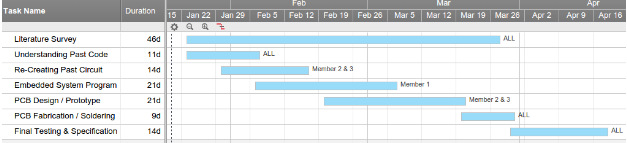
\includegraphics[scale=0.5]{/home/abhin/EDL/EDL/Gantt.png}
\caption{Gantt Chart}
\label{}
\end{figure}
See an HTML version \href{http://publish.smartsheet.com/5856566e76a544e7a8add24073379be7}{here}
\section{Project Implementation}
% At this stage, you need to submit a BOM (Bill of Materials). Apart from the components decide your testing strategy - how to test, needed tools, precautions and feasibility Assessment (resources, risks).  What is the deliverable of the work and demo possible in reality?
\subsection{Components Needed (Bill of Materials)}
\begin{enumerate}
\item \textbf{\href{https://en.wikipedia.org/wiki/Tiva-C_LaunchPad}{Tiva-C LaunchPad}} - Available in WEL Lab to the best of our knowledge.
\item \textbf{\href{http://gnuradio.org/}{GNURadio}} - Free, Open Source Software.
\item \textbf{\href{https://en.wikipedia.org/wiki/Digital-to-analog_converter}{Digital to Analog Converters}} - Basic converters are available in the lab. The more
advanced converters might need to be purchased (To be finalized in literature survey).
\item \textbf{PCB Fabrication Cost}
\end{enumerate}
\subsection{Testing Procedures}
\begin{enumerate}
\item \textbf{DSO Testing} - We intend to keep the frequency of the GNURadio signal as the independent variable. We will try to provide different inputs to the microcontroller and see the output on a DSO.
\item \textbf{Testing with IQ Modulator} - We intend to interface this with an IQ Modulator board and verify whether the produced signal is being transmitted correctly. This will ensure that our device has a working final application and can help us identify additional problems with the circuit.
\end{enumerate}
\section{Deliverables}
% Spell out the project deliverables - what you would demonstrate during the evaluations
% (It is expected that for the first evaluation (1st week of Feb) roughly 30% of work is ready. You will have to demonstrate the subsystems that are ready. For the second evaluation (2nd week of March) 60 to 80% of your work should be over and you should be working on your final PCB, box etc. We expect a draft version of your final report submitted by the 1st week of April. For the final evaluation (April 10-14) you need to give a brief presentation (20 min) and a demo of your project.)

\begin{itemize}
\item \textbf{First Evaluation (mid February)} - Get a working prototype, by recreating most of the past work. Besides this, we hope to have understood TIVA programming well.
\item \textbf{Second Evaluation (mid March)} - Half complete PCB design, final working prototype
\item \textbf{Final Evaluation (mid April)} - Working PCB chip, interfaced with the IQ Modulator board.
\end{itemize}


\end{document}

